% Digital Logic Report Template
% Created: 2020-01-10, John Miller
%==========================================================
%=========== Document Setup  ==============================
% Formatting defined by class file
\documentclass[11pt]{article}
% ---- Document formatting ----
\usepackage[margin=1in]{geometry}  % Narrower margins
\usepackage{booktabs}                    % Nice formatting of tables
\usepackage{graphicx}                    % Ability to include graphics
%\setlength\parindent{0pt}    % Do not indent first line of paragraphs 
\usepackage[parfill]{parskip}      % Line space b/w paragraphs
%     parfill option prevents last line of pgrph from being fully justified
% Parskip package adds too much space around titles, fix with this
\RequirePackage{titlesec}
\titlespacing\section{0pt}{8pt plus 4pt minus 2pt}{3pt plus 2pt minus 2pt}
\titlespacing\subsection{0pt}{4pt plus 4pt minus 2pt}{-2pt plus 2pt minus 2pt}
\titlespacing\subsubsection{0pt}{2pt plus 4pt minus 2pt}{-6pt plus 2pt minus 2pt}
% ---- Hyperlinks ----
\usepackage[colorlinks=true,urlcolor=blue]{hyperref} % For URL's. Automatically 
%links internal references.
% ---- Code listings ----
\usepackage{listings}                          % Nice code layout and inclusion
\usepackage[usenames,dvipsnames]{xcolor} % Colors (needs to be defined before 
%using colors)
% Define custom colors for listings
\definecolor{listinggray}{gray}{0.98}          % Listings background color
\definecolor{rulegray}{gray}{0.7}              % Listings rule/frame color
% Style for Verilog
\lstdefinestyle{Verilog}{
language=Verilog,                        % Verilog
backgroundcolor=\color{listinggray},     % light gray background
rulecolor=\color{blue},                  % blue frame lines
frame=tb,
% lines above & below
linewidth=\columnwidth,                  % set line width
basicstyle=\small\ttfamily,   % basic font style that is used for the code
breaklines=true,                         % allow breaking across 
%columns/pages
tabsize=3,
% set tab size
commentstyle=\color{gray},    % comments in italic 
stringstyle=\upshape,                    % strings are printed in normal 
%font
showspaces=false,                        % don't underscore spaces
}
% How to use: \Verilog[listing_options]{file}
\newcommand{\Verilog}[2][]{%
\lstinputlisting[style=Verilog,#1]{#2}
}







%======================================================
%=========== Body  ====================================
\begin{document}
\title{ELC 2137 Lab 11: FSM: Guessing Game}
\author{Justin Woods}
\maketitle

\section*{Summary}
	In this lab, a finite state machine(FSM) was created. This required the use of sequential logic, but in a way that does not produce repeating patterns. First, a debounce module was created so that when the Basys3 buttons are pressed, the output does not cycle. Thus, the input is held. Then, a guessing game module was created using the same usage of states, but in a way that produces an output appropriate for a guessing game. These two modules were instantiated in a top level module implemented into the Basys3 board, tested by gameplay. 

\section*{Questions}

\begin{enumerate}
	\item At what time in the simulation did the de-bounce circuit reach each of the four states
	
	After 200ns, it would change states. It went from zero to wait1 at 220ns, wait1 to one at 420ns, and one to wait0 at 620ns.
	
	\item Why  can  this  game  not  be  implemented with regular sequential logic?
	
	We cannot use regular sequential logic because the output is not regular, or repeating. We designed an element that can handle non-repeating conditions by creating several states that the input can but the element in. 

	\item What type of outputs did you use for your design (Mealy or Moore)?  Explain.
	
	I used Moore outputs in my design. We see this in that the values of the output are synchronized with the clock, updating at the positive edge, and resetting at the negative edge. This way, only the present state of the machine can change the output.  

\end{enumerate}
\clearpage
\section*{Results}

\begin{figure}[ht]\centering
	\begin{tabular}{l|rrrrrrrr}	
		Time (ns): & 0-100 & 100-200 & 200-300 & 300-400 & 400-500 & 500-600 & 600-700 & 700 -800 \\
		\midrule
		clk     & 0-1 & 0-1 & 0-1 & 0-1 & 0-1 & 0-1 & 0-1 & 0-1 \\
		in  	& 0-1 & 0-1 & 1   & 1   & 1-0 & 1-0 & 0   & 0 \\
		rst 	& 0-1 & 1   & 0   & 0   & 0	  & 0   & 0   & 0 \\
		\midrule
		out 	& X-0 & 0   & 0-1 & 1   & 1   & 1   & 1-0 & 0 \\
		tick	& 0   & 0   & 0-1 & 0   & 0   & 0   & 0	  & 0 \\
		\bottomrule
	\end{tabular}
	\bigskip
	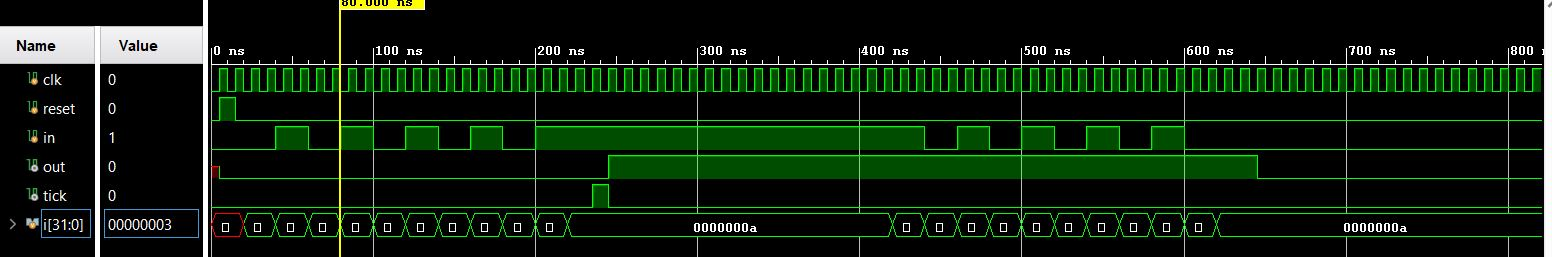
\includegraphics[width=1\textwidth,angle=0,origin=c]{bounce2Waveform}
	\caption{Debounce Waveform with ERT}
	\label{fig:sim_with_table}
\end{figure}

\begin{figure}[ht]\centering
	\begin{tabular}{l|rrrrrrrrr}	
		Time (ns): & 0-10 & 10-20 & 20-30 & 30-40 & 40-50 & 50-60 & 60-70 & 70-80 & 80-90\\
		\midrule
		clk     & 0-1 & 0-1 & 0-1 & 0-1 & 0-1 & 0-1 & 0-1 & 0-1 & 0-1 \\
		rst 	& 0   & 1-0 & 0   & 0   & 0	  & 0   & 0   & 0   & 0 \\
		\midrule
		b 		& 0   & 0   & 4   & 0   & 1   & 0   & 0	  & 0   & 0 \\
		win		& 0   & 0   & 0   & 0   & 0-1 & 1-0 & 0   & 0   & 0 \\
		lose 	& 0   & 0   & 0-1 & 1-0 & 0   & 0   & 0   & 0   & 0 \\
		y 		& f   & e-d & d-f & f-e & e-f & f-e & e-d & d-b & b-7 \\
		\bottomrule
	\end{tabular}
	\bigskip
	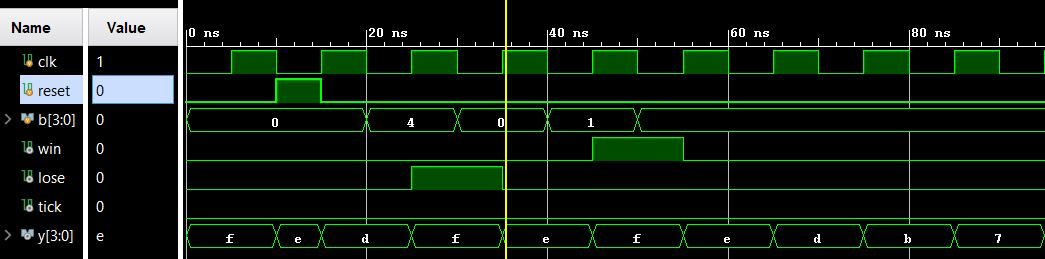
\includegraphics[width=1\textwidth,angle=0,origin=c]{guessFSMwaveform}
	\caption{GuessFSM Waveform with ERT}
	\label{fig:sim_with_table}
\end{figure}

\begin{figure}[ht]\centering
	\begin{tabular}{l|rrrrrrrr}
		Time (ms): & 0-100 & 100-200 & 200-300 & 300-400 & 400-500 & 500-600 & 600-700 & 700 -800 \\
		\midrule
		btnC & 0-1 & 0   & 0      & 0   & 0-1 & 0   & 0      & 0    \\
		btnU & 0   & 1-0 & 0      & 0   & 0   & 1-0 & 0      & 0    \\ 
		btnL & 0-1 & 0   & 0      & 0   & 0-1 & 0   & 0      & 0    \\ 
		btnR & 0   & 0   & 0-1    & 0   & 0   & 0   & 0-1    & 0     \\ 
		btnD & 0   & 0   & 0      & 0-1 & 0   & 0   & 0      & 0-1   \\ 
		sw
		\midrule
		seg   & 7e-7d & 7d-7f & 7f & 7f & 7f & 7f & 7f & 7f \\
		an    & b& e  & e&e& e  & e&e& e \\
		led    & 0000  & 0000-8000   & 8000   & 8000   & 0000-4000 &   0-8000 &0000-8000   & 0000-8000  \\ 
		\bottomrule
	\end{tabular}
	\bigskip
	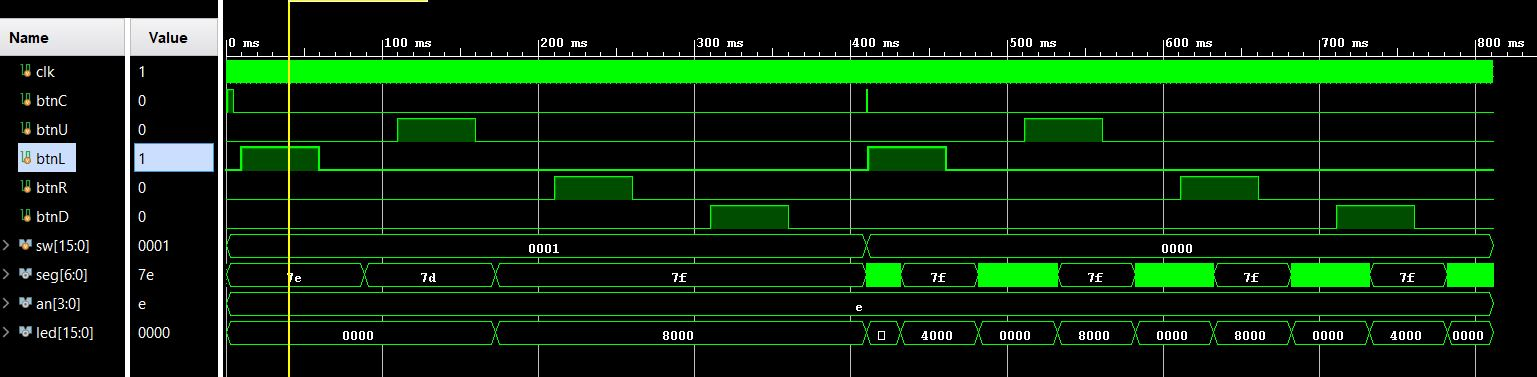
\includegraphics[width=1\textwidth,angle=0,origin=c]{guessinggameWaveform}
	\caption{GuessingGame Waveform with ERT}
	\label{fig:sim_with_table}
\end{figure}

\begin{figure}[ht]\centering
	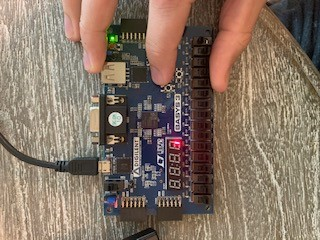
\includegraphics[width=1\textwidth,trim =0 0 0 0,clip,angle=90,origin=c]{slowgameRun}
	\caption{Slow Game Run}
	\label{fig:sim_with_table}
\end{figure}
\begin{figure}[ht]\centering
	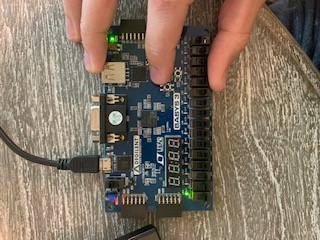
\includegraphics[width=1\textwidth,trim =0 0 0 0,clip, angle=90,origin=c]{slowgameG}
	\caption{Slow Game Guess}
	\label{fig:sim_with_table}
\end{figure}
\begin{figure}[ht]\centering
	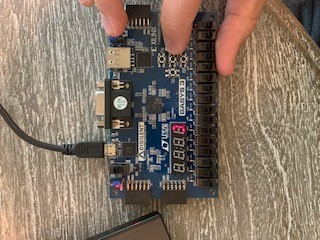
\includegraphics[width=1\textwidth,trim =0 0 0 0,clip, angle=90,origin=c]{fastGamerun}
	\caption{Fast Game Run}
	\label{fig:sim_with_table}
\end{figure}

\begin{figure}[ht]\centering
	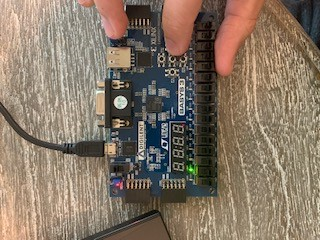
\includegraphics[width=1\textwidth,trim =0 0 0 0,clip,angle=90,origin=c]{fastgameGuess}
	\caption{Fast Game Guess}
	\label{fig:sim_with_table}
\end{figure}

\clearpage
\section*{Code}

\begin{lstlisting}[style=Verilog,
caption=guessFSM,
label=MUX w/ two inputs Source Code
]
module guess_FSM  #( parameter N = 21)
	(input clk , reset ,
	input  [3:0] b,
	output  reg win, lose, [3:0]y,
	output  reg  tick);
	
	//  define  states  as local  parameters (constants)
	localparam  [2:0]
		s0    = 3'b000,
		s1    = 2'b001,
		s2    = 2'b010,
		s3    = 2'b011,
		swin =  3'b100,
		slose = 3'b101;
	
	//  internal  signals
	reg  [2:0]  state , state_next;
	
	// state  memory (register)
	always_ff @(posedge  clk or  posedge reset)
		if (reset) begin
			state    <= s0;
		end
		else  begin
			state    <= state_next;
		end
	
	//  combined  next -state  and  output logic
	always_comb  begin
		//  default  behavior
		state_next    = state;
		tick = 0;
		win = 0;
		lose = 0;
		y = 4'b1111;
		
		case(state)
			s0: begin
				y[0] = 0;                   //Light
				if (!b[3] && !b[2] && !b[1] && b[0]) //Correct button
					state_next = swin;
				else if (b[3] || b[2] || b[1]) //Incorrect button
					state_next = slose;
				else if (!b[3] && !b[2] && !b[1] && !b[0]) //No button
					state_next = s1;
			end
			
			s1: begin
				y[1] = 0;                   //Light
				if (!b[3] && !b[2] && b[1] && !b[0]) //Correct button
					state_next = swin;
				else if (b[3] || b[2] || b[0]) //Incorrect button
					state_next = slose;
				else if (!b[3] && !b[2] && !b[1] && !b[0]) //No button
					state_next = s2;
			end
			
			s2: begin
				y[2] = 0;                  //Light
				if (!b[3] && b[2] && !b[1] && !b[0]) //Correct button
					state_next = swin;
				else if (b[3] || b[1] || b[0]) //Incorrect button
					state_next = slose;
				else if (!b[3] && !b[2] && !b[1] && !b[0]) //No button
					state_next = s3;
			end
			
			s3: begin
				y[3] = 0;
				if (b[3] && !b[2] && !b[1] && !b[0]) //Correct button
					state_next = swin;
				else if (b[2] || b[1] || b[0]) //Incorrect button
					state_next = slose;
				else if (!b[3] && !b[2] && !b[1] && !b[0]) //No button
					state_next = s0;
			end
			
			swin: begin
				win = 1;
				if (!b[3] && !b[2] && !b[1] && !b[0]) //No button
					state_next = s0;
				else if (b[3] || b[2] || b[1] || b[0]) //Any button
					state_next = swin;
			end
			
			slose: begin
				lose = 1;
				if (!b[3] && !b[2] && !b[1] && !b[0]) //No button
					state_next = s0;
				else if (b[3] || b[2] || b[1] || b[0]) //Any button
					state_next = slose;
			end
			
		endcase
	end
endmodule
	
\end{lstlisting}
\clearpage

\begin{lstlisting}[style=Verilog,
caption=guessFSM Test,
label=MUX2 Test
]
module guess_FSMTEST();
	
	reg clk , reset;
	reg [3:0]b;
	wire win, lose, tick;
	wire [3:0]y;
	
	guess_FSM  #(.N(3)) gfms (.clk(clk),
		.reset(reset), .b(b), .win(win), .lose(lose),
		.y(y), .tick(tick));
	
	always  begin
		#5 clk = ~clk;
	end
	
	initial  begin
		clk =0; reset = 0; b = 4'b0000; #10;
		reset = 1; #5;
		reset = 0; #5;
	
		b[2] = 1; #10; b[2] = 0; #10;
		b[0] = 1; #10; b[0] = 0; #10;
	
		$finish;
	end
endmodule  
	
\end{lstlisting}

\begin{lstlisting}[style=Verilog,
caption= guessinggame Source Code,
label=MUX w/ four inputs Source Code
]
module guessing_game
	(input clk, btnC, btnU, btnL, btnR, btnD,
	 input [15:0]sw,
	 output [6:0]seg, [3:0]an, [15:0]led
	);
	
	wire [3:0] dataForGuess;
	wire userTime, toMux, winout, loseout;
	
	debounce  #(.N(21)) d1 (.clk(clk),
		.reset(btnC), .in(btnU), .out(dataForGuess[0]),
		.tick());
	
	debounce  #(.N(21)) d2 (.clk(clk),
		.reset(btnC), .in(btnL), .out(dataForGuess[1]),
		.tick());
	
	debounce  #(.N(21)) d3 (.clk(clk),
		.reset(btnC), .in(btnR), .out(dataForGuess[2]),
		.tick());
	
	debounce  #(.N(21)) d4 (.clk(clk),
		.reset(btnC), .in(btnD), .out(dataForGuess[3]),
		.tick());
	
	counter #(.N(23)) count (.clk(clk),
		.rst(btnC), .en(1'b1), .count(), .tick(toMux));
	
	mux2 #(.N(1)) m1 (.in1(toMux), .in0(clk),
		.sel(sw[0]), .out(userTime));
	
	guess_FSM  #(.N(3)) gfms (.clk(userTime),
		.reset(btnC), .b(dataForGuess), .win(winout), .lose(loseout),
		.y(seg[3:0]), .tick());
	
	assign an[3:0] = 4'b1110;
	assign seg[6:4] = 3'b111;
	assign led[13:0] = 0;
	assign led[14] = winout;
	assign led[15] = loseout;

endmodule
	
\end{lstlisting}
\clearpage
\begin{lstlisting}[style=Verilog,
caption=guessinggame Test,
label=MUX4 Test
]	
module guessing_gameTEST();
	
	reg clk, btnC, btnU, btnL, btnR, btnD;
	reg [15:0]sw;
	wire [6:0]seg;
	wire [3:0]an;
	wire [15:0]led;
	
	guessing_game gg (.clk(clk), .sw(sw), 
		.btnC(btnC), .btnU(btnU), .btnL(btnL),
		.btnR(btnR), .btnD(btnD), .seg(seg), 
		.an(an), .led(led));
	
	always  begin
		#5 clk = ~clk;
	end
	
	
	initial  begin
		clk = 0; 
		sw = 1;
		btnC = 0; btnU = 0; btnL = 0; btnR = 0; btnD = 0;
		#10;
	
		btnC = 1; #5000000;
		btnC = 0; #5000000;
		
		btnL = 1; #50000000 btnL = 0; #50000000;
		btnU = 1; #50000000 btnU = 0; #50000000;
		btnR = 1; #50000000 btnR = 0; #50000000;
		btnD = 1; #50000000 btnD = 0; #50000000;
		
		sw = 0;
		btnC = 1; #500000;
		btnC = 0; #500000;
		
		btnL = 1; #50000000 btnL = 0; #50000000;
		btnU = 1; #50000000 btnU = 0; #50000000;
		btnR = 1; #50000000 btnR = 0; #50000000;
		btnD = 1; #50000000 btnD = 0; #50000000;
	
		$finish;
	end     
endmodule
\end{lstlisting}

\end{document}